Para criar um logotipo, um profissional da �rea de design gr�fico deseja constru�-lo utilizando o conjunto de pontos do plano na forma de um tri�ngulo, exatamente como mostra a imagem. 

\begin{figure}[h]
\centering
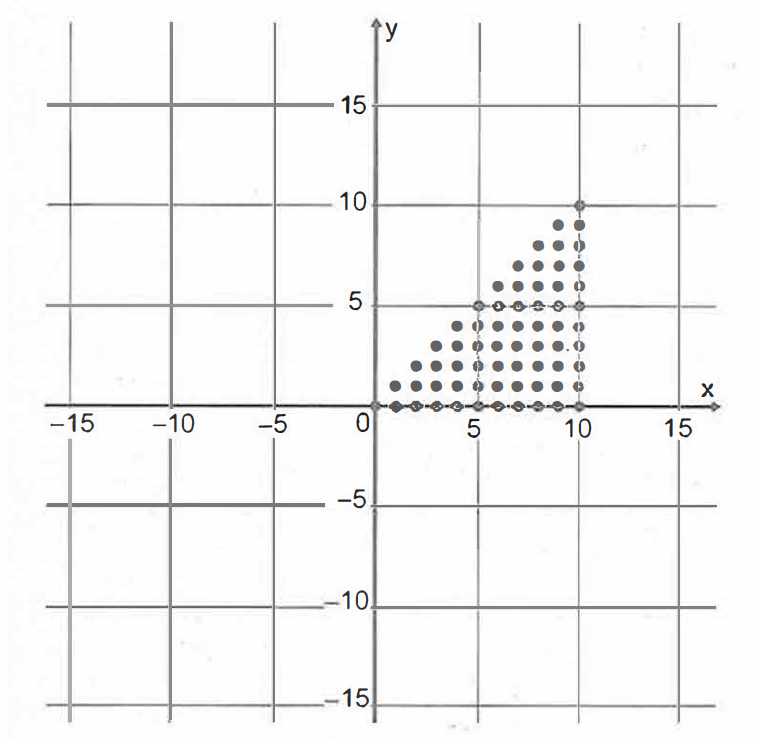
\includegraphics[width=8cm]{../figuras/q158-2018.png}
\end{figure}

Para construir tal imagem utilizando uma ferramenta gr�fica, ser� necess�rio escrever algebricamente o conjunto que representa os pontos desse gr�fico. 
Esse conjunto � dado pelos pares ordenados $(x; y) EN \times N$, tais que 

\begin{enumerate}
\item[a)]$0\leq x \leq y \leq 10$
\item[b)]$0\leq y \leq x \leq 10$
\item[c)]$0\leq x \leq 10,\ 0\leq y \leq 10$
\item[d)]$0\leq x+ y \leq 10$
\item[e)]$0\leq x +y \leq 20$
\end{enumerate}